\scanpage{3}
\figure{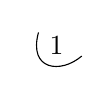
\begin{tikzpicture}[x=1cm,y=1cm]\node at (0,0) {\mspage{1}};\draw (-.23,.17) .. controls (-.36,-.31) and (.05,-.36) .. (.32,-.13);\end{tikzpicture}}
\uline{Théorème} $S$ schéma loc. noeth, $U$ ouvert, $T$ fermé complémentaire,
$p$ \unsure{ent} premier, tel que $\forall t\in T$, $\operatorname{car}k(t)=p$. Considérons la
catégorie $C$ des schémas abéliens \inserted{$A$} sur $S$, et la catégorie $C'$ des
couples $(A_U,M,\varphi)$, où $A_U$ est un schéma abélien sur $U$, $M$
un \unsure{grpe|groupe} $p$-divisible sur $S$, et $\varphi:M|U\longrightarrow T_p(A_U)$. Soit
\[F:C\longrightarrow C'\]
le foncteur
\[F(A)=(A\times_S U,T_p(A),\operatorname{id}_{T_p(A)|U}).\]
Alors:

1) Supposons que $U$ rencontre ttes composantes connexes
de $S$. \inserted{(\unsure{p.ex.} $U$ dense dans $S$, i.e. $\operatorname{prof\,et}_T(S)\geq1$).} Alors le foncteur $F$ est pleinement fidèle.

2) Supposons que \deleted{$U$ soit dense dans $S$, et que}
\inserted{a) $\exists$ morphisme fini surjectif $S'\longrightarrow S$, avec $S'$ géom. unibranche (\unsure{p.ex. la normalisée} de $S$ est finie sur $S$, si $S$ local).}
\deleted{\inserted{b)} pour tout $t\in T$, si $S'$ est le localisé strict de $S$ en $t$,
\inserted{($\bar t$ son point fermé)} et $S'_1$ et $S'_2$ deux composantes irréductibles de $S'$, on ait
\[S'_1\cap S'_2\ne\{\bar t\}.\]
(NB. Cette condition équivaut aussi à celle-ci:
\deleted{\unsure{dans un} \illegible{2}} l'image inverse $U''$ de $U$ dans $S''=S'\times_S S'$
\deleted{équivalence de catégories} \unsure{est dense dans} $S''$. \unsure{Et $U$ est} \unsure{un} \illegible{1} \deleted{\unsure{strict}} \unsure{géom. connexe}
\unsure{en un point de} $T$) Alors \deleted{b) Posant}}
\inserted{b) On a $\operatorname{prof\,et}_T(S)\geq2$ \unsure{\S}.}
Alors $F$ est \deleted{pleinement fidèle}\inserted{une équivalence des catégories}.
\margin{\figure{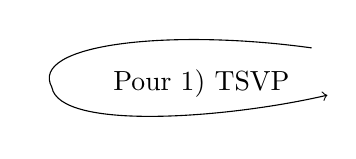
\begin{tikzpicture}[x=1cm,y=1cm]
\node at (1.7,0) {Pour 1) TSVP};
\draw[->] (3.1,.45) .. controls (1.3,.7) and (-.5,.5) .. (-.2,-.05) .. controls (-.1,-.6) and (2,-.45) .. (3.3,-.15);
\end{tikzpicture}}}

\margin{$\S$ Soit, avec les notations de a), $S''=S'\times_S S'$, $S'''=S'\times_S S'\times_S S'$. Considérons
l'ensemble simplicial
\diagram{\begin{tikzcd}[column sep=large,row sep=small]
\inserted{L_0} \arrow[d,phantom,"\unsure{\Vert}" description] & \inserted{L_1} \arrow[d,phantom,"\unsure{\Vert}" description] & \inserted{L_2} \arrow[d,phantom,"\unsure{\Vert}" description] \\
\pi_0(S') & \pi_0(S'') \arrow[l,shift left=.6ex] \arrow[l,shift right=.6ex] & \pi_0(S''') \arrow[l,shift left=1ex] \arrow[l] \arrow[l,shift right=1ex]
\end{tikzcd}}, \deleted{\unsure{les}} et \deleted{soit}
soit
\diagram{\begin{tikzcd}K_0 & K_1 \arrow[l,shift left=.6ex] \arrow[l,shift right=.6ex] & K_2 \arrow[l,shift left=1ex] \arrow[l] \arrow[l,shift right=1ex]\end{tikzcd}}
le ss-ensemble simplicial formé avec
les composantes connexes dont l'image dans $S$ rencontre $U$.
Supposons\unsure{:} \unsure{que:} \deleted{pour tout}\inserted{b')} la plus petite partie de $L_1$
contenant $K_1$ et stable par ``troisième face'' soit $L_1$ (c'est
ce qui est assuré par la condition b)). Alors $F$ est \deleted{\unsure{pl. fid.}}
\inserted{une} équivalence de catégories $\ldots\ldots$.}
\mspage{2}
